\documentclass{beamer}
\usetheme{Warsaw}
\setbeamertemplate{footline}[frame number]
\usepackage[utf8]{inputenc}
\usepackage{fancybox}
\usepackage{multimedia} 
\usepackage{subfig}
\usepackage{amsmath}
\usepackage{hyperref}
\usepackage[all]{xy}
\begin{document}


\title[Angewandte Mathematik] % (optional, only for long titles)
{Angewandte Mathematik
\\
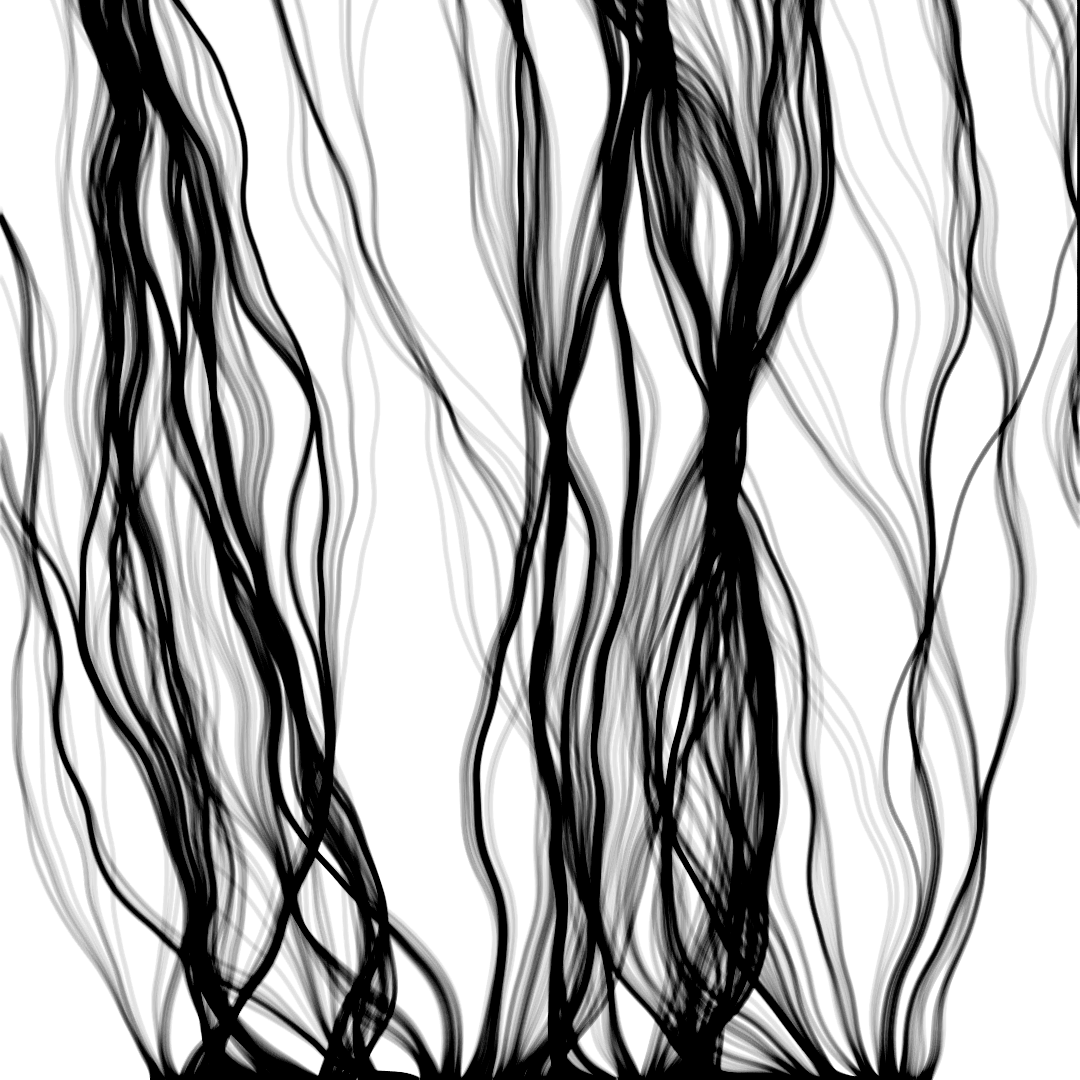
\includegraphics[scale=0.15]{images/cover}
}
\subtitle{}
\author[Dr. Johannes Riesterer] % (optional, for multiple authors)
{Dr.  rer. nat. Johannes Riesterer}

\date[KPT 2004] % (optional)
{}

\subject{Angewandte Mathematik}



\begin{frame}
    \frametitle{Angewandte Mathematik}
\framesubtitle{Kettenregel}

    \begin{block}{Mehrdimensionale Differenzierbarkeit}
Für $z:= (z_1, \cdots ,z_k) \in \mathbb{R}^k$ bezeichnen 
\begin{align*}
& pr_i : \mathbb{R}^k \to \mathbb{R} \\
& pr_i(z): = <e_i, z>_2 = z_i
\end{align*}
die Projektionen auf die $i$-te Koordinate.
\end{block}


    \begin{block}{Mehrdimensionale Differenzierbarkeit}
Für zwei Funktionen  $g: U \subset \mathbb{R}^n \to V  \subset \mathbb{R}^m$ und $f: V \subset \mathbb{R}^m \to W  \subset \mathbb{R}^l$ bezeichnet 
\begin{align*}
& f \circ g: U \to W \\
& (f \circ g)(x) : = f (g(x))
\end{align*}
die Hintereinanderausführung (Verkettung) von $f$ und $g$.
\end{block}

 \end{frame}





\begin{frame}
    \frametitle{Angewandte Mathematik}
\framesubtitle{Kettenregel}

    \begin{block}{Mehrdimensionale Differenzierbarkeit}
Eine Funktion $F: U \subset \mathbb{R}^n \to \mathbb{R}^m$ ist genau dann differenzierbar, wenn alle Koordinatenfunktionen
\begin{align*}
& F_i :U \subset \mathbb{R}^n \to \mathbb{R} \\
& F_i(x): = (pr_i \circ F) (x) := pr_i(F(x))
\end{align*}
differenzierbar sind.
\end{block}

 \end{frame}



\begin{frame}
    \frametitle{Angewandte Mathematik}
\framesubtitle{Kettenregel}

    \begin{block}{Beweis}
Betrachte $dF = (dF_1, \cdots, dF_m) $ zusammen mit dem  Restglied $R(h)  = (R_1(h), \cdots, R_m(h))$ definiert jeweils durch die rechte oder linke Seite.
\end{block}

 \end{frame}




\begin{frame}
    \frametitle{Angewandte Mathematik}
\framesubtitle{Kettenregel}
\begin{block}{Kettenregel}
Sind $g: U \subset \mathbb{R}^n \to V  \subset \mathbb{R}^m$ und $f: V \subset \mathbb{R}^m \to W  \subset \mathbb{R}^l$ differenzierbar, so ist $g \circ f$ differenzierbar und es gilt
\begin{align*}
d(f \circ g)(a) = df(b) \cdot dg(a)
\end{align*}
mit $b = g(a)$.
\end{block}

 \end{frame}



\begin{frame}
    \frametitle{Angewandte Mathematik}
\framesubtitle{Kettenregel}
    \begin{block}{Beweis}
Nach Voraussetzung gilt
\begin{align*}
g(a + h) = g(a) + dg(a)h + ||h||r_1(h);  \; \; \lim_{h \to 0} r_1(h) = 0\\
f(b + k) = f(b) + df(b)k + ||k||r_2(k); \; \; \lim_{k \to 0} r_1(k) = 0
\end{align*}
\end{block}

    \begin{block}{Beweis Kettenregel}
Einsetzten ergibt 
\begin{align*}
(f \circ g)(a + h) = (f \circ g)(a)  + (df(b) \cdot dg(a) )h + R(h)
\end{align*}
mit $R(h):= ||h|| df(b) r_1(h) + ||k|| r_2(k)$  und $k= dg(a)h + ||h||r_1(h)$.
\end{block}
 \end{frame}



\begin{frame}
    \frametitle{Angewandte Mathematik}
\framesubtitle{Kettenregel}
    \begin{block}{Beweis Kettenregel}
Müssen nur noch zeigen, dass $\lim_{h \to 0} \frac{R(h)}{||h||} = 0$ gilt.

\end{block}

    \begin{block}{Beweis Kettenregel}
Da $dg(a)$ eine lineare Abbildung ist, gibt es ein $c \in \mathbb{R}$ mit 
\begin{align*}
||k|| \leq ||h|| (c + || r_1(h)||)
\end{align*}
womit die Behauptung folgt.
\end{block}



 \end{frame}





\begin{frame}
    \frametitle{Angewandte Mathematik}
\framesubtitle{Vertauschen von Ableitungen}
    \begin{block}{Satz von Schwarz}
Wenn Für eine Funktion $f: U \to \mathbb{R}$ die Ableitungen $\frac{\partial}{\partial x_i} f(a)$, $\frac{\partial}{\partial x_j}f(a)$ und $ \frac{\partial}{\partial x_i}\frac{\partial }{\partial x_j} f(a)$ existieren und letztere stetig ist, dann existiert auch $ \frac{\partial}{\partial x_j}\frac{\partial }{\partial x_i} f(a)$ und es gilt
\begin{align*}
\frac{\partial}{\partial x_i}\frac{\partial }{\partial x_j} f(a) = \frac{\partial}{\partial x_j}\frac{\partial }{\partial x_i} f(a)
\end{align*}
\end{block}
    \begin{block}{Bedeutung}
Die Reihenfolge spielt beim wiederholten ableiten keine Rolle.
\end{block}
 \end{frame}



\begin{frame}
    \frametitle{Angewandte Mathematik}
\framesubtitle{Höhere Ableitungen}
    \begin{block}{$\mathcal{C}^k$-Funktionen}
Eine  Funktion  $f: U \to \mathbb{R}$ für die alle partiellen Ableitungen 
\begin{align*}
 \frac{\partial}{\partial x_{i_1}} \cdots   \frac{\partial}{\partial x_{i_k}} f(a)
\end{align*}
mit $ i_1 +  \cdots + i_k \leq k$ existieren und stetig sind heißt $\mathcal{C}^k$-Funktion oder $k$-mal stetig differenzierbar.
\end{block}
    \begin{block}{$\mathcal{C}^k$-Funktionen}
 Eine  $\mathcal{C}^1$-Funktion ist also eine differenzierbare Funktion.
\end{block}
 \end{frame}


\begin{frame}
    \frametitle{Angewandte Mathematik}
\framesubtitle{Höhere Ableitungen}
    \begin{block}{p-te Ableitung}
Für  eine Funktion  $f: U \to \mathbb{R}$, $a \in U$ und Vektoren $v^1, \cdots , v^p \in \mathbb{R}^n$ heißt 
\begin{align*}
d^pf(a) \bigl(v^1, \cdots , v^p  ) := \partial_{v^1} \hdots \partial_{v^p} f(a)
\end{align*}
die $p$-te Richtungsableitung von $f$. Sie ist wegen dem Satz von Schwarz wohldefiniert.

\end{block}
    \begin{block}{}
\begin{align*}
d^pf(a) \bigl(v^1, \cdots , v^p  ) = \sum_{i_1 = 1}^n \cdots \sum_{i_p = 1}^n  \frac{\partial}{\partial x_{i_1}} \hdots \frac{\partial}{\partial x_{i_p}} f(a) \cdot v^1_{i_1} \cdots v^p_{i_p} \; .
\end{align*}
Für einen Vektor $z \in \mathbb{R}^n$ definieren wir $d^pf(a) z^p := d^pf(a) \underbrace{(z, \cdots , z)}_{p-mal} \;.$

\end{block}
 \end{frame}


\begin{frame}
    \frametitle{Angewandte Mathematik}
\framesubtitle{Höhere Ableitungen}
    \begin{block}{Hessematrix}
Für $p = 2$ und $u,v \in \mathbb{R}^n$ ist
\begin{align*}
d^2f(a) \bigl(u , v ) = \sum_{i = 1}^n \sum_{j = 1}^n \frac{\partial}{\partial x_{i}}  \frac{\partial}{\partial x_{j}} f(a) v_{i}  u_{i} 
\end{align*}
und mit 
\begin{align*}
f''(a) : = \begin{pmatrix}  \frac{\partial}{\partial x_{1}} \frac{\partial}{\partial x_{1}} f(a)   &  \cdots &  \frac{\partial}{\partial x_{1}} \frac{\partial}{\partial x_{n}} f(a) \\
\vdots & & \vdots  \\
 \frac{\partial}{\partial x_{n}} \frac{\partial}{\partial x_{1}} f(a)   &  \cdots &  \frac{\partial}{\partial x_{n}} \frac{\partial}{\partial x_{n}} f(a)
\end{pmatrix} 
\end{align*}
ist $d^2f(a) \bigl(u , v ) = u^T  \cdot f''(a) \cdot v$. Die Matrix $f''(a)$ wird auch Hesse-Matrix genannt. Nach dem Satz von Schwarz ist sie symmetrisch.
\end{block}
 \end{frame}

\begin{frame}
    \frametitle{Angewandte Mathematik}
\framesubtitle{Höhere Ableitungen}
    \begin{block}{Taylorapproximation}
Sei   $f: U \to \mathbb{R}$ eine $\mathcal{C}^{p+1}$-Funktion und $x,a \in U$, so dass die Verbindung zwischen $x$ und $a$ in $U$ liegt.
Dann gilt
\begin{align*}
f(x) = f(a) + \sum_{k=1}^{p}\frac{1}{p!} d^k f(a) (x-a)^k + R_{p+1} (x;a)
\end{align*}
mit dem Restglied $R_{p+1} (x;a) := \frac{1}{(p+1)!} d^{p+1}f(\xi) (x-a)^{p+1}$ für ein $\xi \in [a,x]$.

\end{block}
\begin{block}{Beispiel}
\href{https://de.wikipedia.org/wiki/Taylor-Formel\#Taylor-Formel_im_Mehrdimensionalen}{Wiki}
\end{block}
 \end{frame}


\begin{frame}
    \frametitle{Angewandte Mathematik}
\framesubtitle{Höhere Ableitungen}
    \begin{block}{Beweis}
Sei $F(t) := f(a + th)$ mit $t \in [0,1]$. Wiederholte Anwendung der Kettenregel mit $\gamma(t) := a +th$ und $F(t) = f(\gamma(t))$ ergibt
\begin{align*}
& F'(t) = \sum_{i=1}^n  \frac{\partial}{\partial x_{i}} f(a + th) h_i \\
& F''(t) =\sum_{j=1}^n \sum_{i=1}^n   \frac{\partial}{\partial x_{j}} \frac{\partial}{\partial x_{i}} f(a + th) h_i h_j \\
& \vdots \\
& F^p(t) =  \sum_{i_1=1}^n  \cdots \sum_{i_p=1}^n   \frac{\partial}{\partial x_{i_1}} \cdots \frac{\partial}{\partial x_{i_p}} f(a + th) h_{i_1} \cdots  h_{i_p}  \; .
\end{align*}
\end{block}
 \end{frame}

\begin{frame}
    \frametitle{Angewandte Mathematik}
\framesubtitle{Höhere Ableitungen}
    \begin{block}{Beweis}
Mit der Taylorapproximation für Funktionen einer Veränderlichen  folgt für $h := (x-a)$ 
\begin{align*}
 F(1) = F(0) + F'(0) + \frac{1}{2!} F''(0) + \cdots + \frac{1}{p!} F^p(0) + R_{p+1} 
\end{align*}
mit dem Restglied $ R_{p+1}  :=  \frac{1}{(p+1)!}  F^p(\tau)$ mit $\tau \in [0,1]$.
Da nach Konstruktion $F(0) = f(a)$ und $F(1)= f(x)$ folgt insgesamt die Behauptung.
\end{block}
 \end{frame}

\begin{frame}
    \frametitle{Angewandte Mathematik}
\framesubtitle{Höhere Ableitungen}
    \begin{block}{Taylorapproximation}
Sei $T_p(x,a) =  f(a) + \sum_{k=1}^{p}\frac{1}{p!} d^k f(a) (x-a)^k$ die Taylorraproximation einer $\mathcal{C}^{p}$-Funktion. Dann gilt: 
\begin{align*}
\lim_{x \to a} \frac{f(x) - T_p(x;a)}{  || x-a  ||^p} = 0 \;. 
\end{align*}
\end{block}

    \begin{block}{Bedeutung}
Die Taylorapproximation vom Grad $p$ konvergiert polynominell vom Grad $p$ gegen $0$.
\end{block}
 \end{frame}

\begin{frame}
    \frametitle{Angewandte Mathematik}
\framesubtitle{Höhere Ableitungen}
    \begin{block}{Beweis}
Da die partiellen Ableitungen stetig sind, gibt es für jedes $\epsilon > 0$ ein Radius $r >0$, dass für alle $y \in K_r(a)$
\begin{align*}
\frac{1}{p!} (d^pf(y) -d^pf(a))h^p \leq \epsilon ||h||_{\infty}^p \; . 
\end{align*}
Mit der Taylorapproximation ist 
\begin{align*}
f(x) = & T_{p-1}(x, a) +  \frac{1}{p!} d^{p}f(\xi) (x-a)^{p} \\
 = & T_p(x,a) +   \frac{1}{p!} \bigl( d^pf(\xi) -d^pf(a) \bigr) h^p (x-a)^p
\end{align*} 
Mit obiger Abschätzung folgt die Behauptung.
\end{block}
 \end{frame}


\begin{frame}
    \frametitle{Angewandte Mathematik}
\framesubtitle{Extrema}
    \begin{block}{Extrema}
Sei $f : X \subset \mathbb{R}^n \to \mathbb{R}$ eine relle Funktion.  Ein Punkt $a \in  X$ heißt lokales Maximum bzw. Minimum, falls eine Umgebung $U$ von $a$ existiert, so dass $f(x) \leq f(a)$ bzw.  $f(x) \geq f(a)$ für alle $x \in U$ gilt. Liegt einer der beiden Fälle vor, so spricht man von einem lokalen Extremum. Gilt strikt $f(x) <  f(a)$ bzw.  $f(x) > f(a)$ , so nennt man das Extremum isoliert. Ist $U = X$ so nennt man es auch globales Maximum bzw. Minimum.
\end{block}
 \end{frame}


\begin{frame}
    \frametitle{Angewandte Mathematik}
\framesubtitle{Extrema}

\begin{figure}[H]
      \centering
    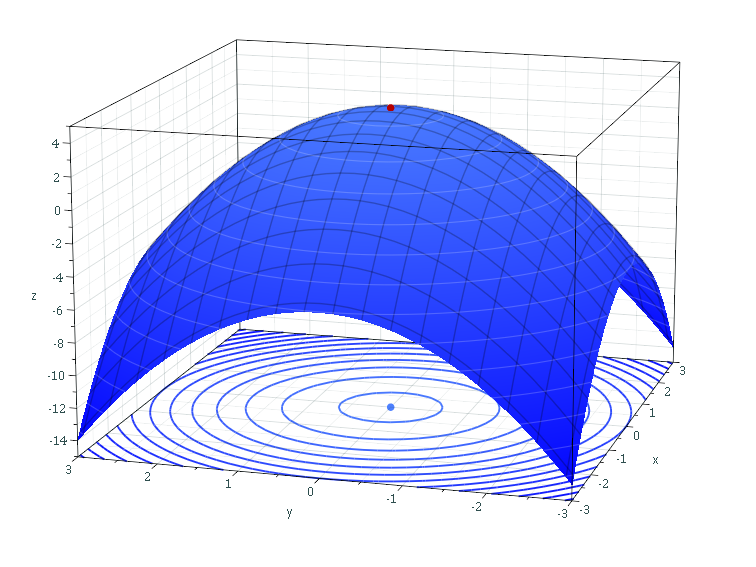
\includegraphics[width=0.8\textwidth]{images/MaximumParaboloid}
      \caption{Quelle: Wikipedia: https://en.wikipedia.org/wiki/File:MaximumParaboloid.png}
   \end{figure}
 \end{frame}

\begin{frame}
    \frametitle{Angewandte Mathematik}
\framesubtitle{Extrema}

\begin{figure}[H]
      \centering
    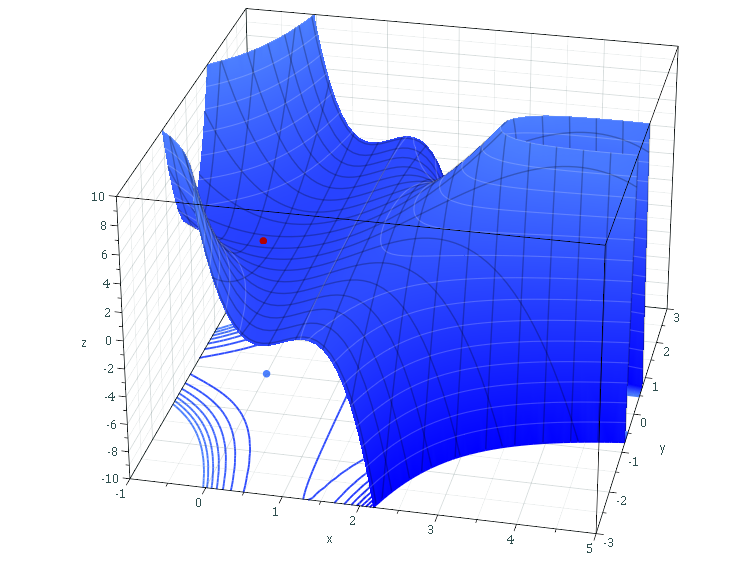
\includegraphics[width=0.8\textwidth]{images/MaximumCounterexample}
      \caption{Quelle: Wikipedia: https://en.wikipedia.org/wiki/File:MaximumCounterexample.png}
\end{figure}
 \end{frame}



\begin{frame}
    \frametitle{Angewandte Mathematik}
\framesubtitle{Extrema}
    \begin{block}{Extrema}
 Ist $f: U  \to \mathbb{R}$ differenzierbar und hat  $f$ in $a \in U$ ein lokales Extremum, so gilt 
\begin{align*}
\frac{\partial}{\partial x_{1}} f(a) = \cdots  = \frac{\partial}{\partial x_{n}} f(a) = 0 \;.
\end{align*}
Sind die partiellen Ableitungen stetig, ist dies  gleichbedeutend mit $df(a) = 0$.
\end{block}
    \begin{block}{Kritischer Punkt}
 Ein Punkt $a$ mit $df(a) = 0$ wird kritischer Punkt genannt.
\end{block}

 \end{frame}

\begin{frame}
    \frametitle{Angewandte Mathematik}
\framesubtitle{Extrema}
    \begin{block}{Beweis}
Setze $F_k(t) := f(a + t e_k)$. Da $f$ ein Extremum in $a$ hat, hat $F_k$ in einer hinreichend kleinen Umgebung um $0$ ein Extremum. 
Da $F_k$ eine Funktion einer Veränderlichen ist, gilt $F'(0) = 0$. Da $\frac{\partial}{\partial x_k} f(a) = F_k'(0)$ folgt die Behauptung.
\end{block}
 \end{frame}


\begin{frame}
    \frametitle{Angewandte Mathematik}
\framesubtitle{Extrema}
    \begin{block}{Extrema}
 Ist $f: U  \to \mathbb{R}$ eine $\mathcal{C}^2$-Funktion und ist $f'(a) = 0$ für ein $a \in U$. Dann gilt:
\begin{itemize}
\item $f''(a) > 0 \Rightarrow $ $f$ hat in $a$ ein isoliertes lokales Minimum.
\item $f''(a) < 0 \Rightarrow $ $f$ hat in $a$ ein isoliertes lokales Maximum.
\item $f''(a) \gtrless 0 \Rightarrow $ $f$ hat in $a$ einen Sattelpunkt.
\end{itemize} 
\end{block}
 \end{frame}


\begin{frame}
    \frametitle{Angewandte Mathematik}
\framesubtitle{Extrema}
    \begin{block}{Extrema}
$f''(a) > 0 \Leftrightarrow x^t f''(a) x > 0 \; \; \forall x \in \mathbb{R}^n \Leftrightarrow \; \; $ alle Eigenwerte sind positiv $\Leftrightarrow$ Alle Hauptminoren sind positiv . 
\end{block}
    \begin{block}{Extrema}
$f''(a) < 0 \Leftrightarrow x^t f''(a) x < 0 \; \; \forall x \in \mathbb{R}^n \Leftrightarrow \; \; $ alle Eigenwerte sind negativ $\Leftrightarrow$ Alle Hauptminoren sind alternierend. 
\end{block}
 \end{frame}



\begin{frame}
    \frametitle{Angewandte Mathematik}
\framesubtitle{Extrema}
    \begin{block}{Beweis}

Sei $f'(a) = 0$ und $f''(a) > 0$. Mit der Taylorformel gilt für hinreichend kurze Vektoren $h \in \mathbb{R}^n$
\begin{align*}
f(a + h) = f(a) + \frac{1}{2} h^T f''(a) h + R(h)
\end{align*}
mit $\lim_{h \to 0} \frac{R(h)}{ ||h||} = 0$. Für $||h|| \leq 1$ hat $ h^T f''(a) h $ sein Maximum $m$ auf dem Einheitskreis $\{ h \in \mathbb{R}^n \; | \; ||h|| = 1 \}$ da $f''(a) > 0$.
\begin{align*}
 h^T f''(a) h  = ||h|| \frac{1}{||h||} h^t  f''(a)  ||h|| \frac{1}{||h||} h \geq m ||h||^2 \;.
\end{align*}
\end{block}
 \end{frame}



\begin{frame}
    \frametitle{Angewandte Mathematik}
\framesubtitle{Extrema}
    \begin{block}{Beweis}
Wir wählen $\epsilon$ so klein, dass $R(h) \leq \frac{m}{2}  ||h||^2$ gilt für $||h|| < \epsilon$  (was geht wegen Taylorformel).
Damit erhalten wir
\begin{align*}
f(a + h) \geq f(a) +  m ||h||^2 \;.
\end{align*}
und damit hat $f$ ein lokales Minimum in $a$.

Der Fall $f''(a) < 0$ wird mit Betrachtung von $-f$ durch den vorigen Fall bewiesen.
\end{block}
 \end{frame}



\begin{frame}
    \frametitle{Angewandte Mathematik}
\framesubtitle{Extrema}
    \begin{block}{Beweis}


Es sei nun $f''(a) \gtrless 0$ und $v$ mit $v^T f''(a) v > 0$ und $w$ mit $w^T f''(a) w > 0$. Betrachten wir die Funktionen
\begin{align*}
F_v (t) := f(a + tv) \\
F_w(t) := f(a +tw)
\end{align*}
dann ist 
\begin{align*}
F_v' (t) = 0; \; F_v''(0) = v^T f''(a) v > 0 \\
F_w' (t) = 0; \; F_w''(0) = w^T f''(a) w < 0 \\
\end{align*}
und somit hat $F_v$ ein isoliertes lokales Maximum und $F_w$ ein isoliertes lokales Minimum und damit $f$ kein lokales Extremum  in  $a$.
\end{block}
 \end{frame}



\begin{frame}
    \frametitle{Angewandte Mathematik}
\framesubtitle{Mittelwertsatz}
    \begin{block}{Mittelwertsatz}
Ist $f: U \to \mathbb{R}$ eine differenziertere Funktion und $a,b \in U$ Punkte, deren Verbindungsstrecke in $U$ verläuft. Dann gibt gibt es einen Punkt $\xi$ auf dieser Verbindungsstrecke mit
\begin{align*}
f(b) - f(a) = df(\xi)(b-a) = f'(\xi) (b-a)
\end{align*}
\end{block}
 \end{frame}



\begin{frame}
    \frametitle{Angewandte Mathematik}
\framesubtitle{Mittelwertsatz}
    \begin{block}{Beweis Mittelwertsatz}
Die Verbindungsstrecke ist gegeben durch $\gamma(t) := a + t(b-a)$ mit $t \in [0,1]$. 
Für $F:= f \circ \gamma : [0,1] \to \mathbb{R}$ gilt $f(b) - f(a)= F(1) - F(0)$.
Nach der Kettenregel ist $F$ differenzierbar. Mit dem eindimensionalen Mittelwertsatz gibt es also ein $\tau \in (0,1)$ mit
$F(1) - F(0) = F'(\tau)$. Mit der Kettenregel folgt $F'(\tau) = df(\gamma(\tau)) (b-a)$ und somit folgt mit $\xi= \gamma(\tau)$ die Behauptung.
\end{block}
 \end{frame}


\end{document}

